\documentclass[11pt]{article}
\usepackage[T1]{fontenc}
\usepackage[utf8]{inputenc}
\usepackage{newpxtext,newpxmath}
\usepackage[textwidth=5.6in,textheight=8.6in]{geometry}
\usepackage{microtype}
\usepackage{booktabs}
\usepackage{graphicx}
\usepackage{float}
\usepackage{parskip}
\usepackage{xcolor}
\definecolor{bindingblue}{HTML}{1668A1}
\usepackage[colorlinks=true,allcolors=bindingblue]{hyperref}
\graphicspath{{../writeup_figures/figures/}}

% tighter spacing: run-in headings sit closer to their text, less vertical
% air above them, and math relations spaced like ordinary words
\makeatletter
\renewcommand\paragraph{\@startsection{paragraph}{4}{\z@}%
  {1.25ex \@plus .5ex \@minus .2ex}%
  {-0.5em}%
  {\normalfont\normalsize\bfseries}}
\makeatother
\thickmuskip=3mu plus 2mu
\medmuskip=3mu plus 1mu minus 2mu
\frenchspacing
\makeatletter
\renewcommand\@seccntformat[1]{\csname the#1\endcsname\hspace{0.6em}}
\makeatother

\title{\LARGE Who Decides When the Task Is Done?\\[3pt]\large Measuring the Effect of Moving Completion Authority\\from LLMs to Checkers}
\author{Kushagra Bhatnagar\\
\small\url{https://github.com/kushagrab21/binding-feedback-experiment}}
\date{July 2026}

\begin{document}
\maketitle

\section*{\centering Abstract}

\noindent An LLM agent finishes a task in one of two ways: either the model judges its own work complete, which we call advisory feedback, or a checker computes completion and the model's claim carries no authority, which we call binding feedback. The distinction matters because an LLM is a generator rather than a verifier. When the specification is incomplete, it fills the gap from its priors, grades its work against that reconstructed answer key, and can confidently declare wrong work finished. We call this failure the false-DONE: the model does not know when it does not know. Across three preregistered experiments on frozen buggy-Python repair corpora, 2,862 episodes over seven models from five providers at under one dollar of total compute, we isolate this authority placement as the only varying factor. Binding lifts a weak model by 9.2 points while leaving a strong one unchanged. Across a seven-model capability ladder the gain is a window, peaking mid-ladder at +14.9 points, zero at the ceiling, and negative for the weakest model, which fails by thrashing rather than false claiming. Raising task difficulty by composing two and three simultaneous bugs roughly doubles the window's depth, up to +31.7 points, but never moves its ceiling: the strongest model produces zero false claims at every difficulty. The window is therefore a property of the model, not the model--task pair, and the advisory false-DONE rate mediates the entire effect, which makes the intervention predictable: a short probe that counts false claims tells a designer in advance whether completion gating will pay.



\setcounter{section}{1}
\section{Question}

This work began with a practical frustration. I was building an agent that wrote programs in a domain-specific language and repaired them using compiler feedback. The feedback arrived as text, and the model routinely failed to act on it: it would acknowledge an error and then resubmit the same code, or fall back to what its priors suggested, or simply give up. I first tried managing the agent's context so that the important feedback stayed at high priority, but the model still ignored it often enough to be unreliable. That failure changed the question I was asking. Instead of asking how to phrase feedback so that the model listens, I asked what happens if listening is no longer optional, that is, if the guarantee is moved out of the prompt and into the infrastructure that delivers the feedback.

The experiment compares two agent designs on a simple repair task. The model is given a short Python function into which exactly one bug has been introduced by changing a single line, and its job is to correct the code. The function is presented bare: its description, docstrings, and comments have been stripped beforehand, so the model cannot read what the code is supposed to do. The only way for the model to recover the missing specification is to submit code and learn from the checker's feedback. The two designs are identical in every respect except one. In both, the model submits code, a checker executes the task's tests, and the verdict is returned to the model as feedback, with the feedback text byte-identical across the two designs. The difference is who holds the authority to end the episode. In advisory mode, the model may declare the task done, and the declaration is believed even when the last verdict was FAILED. In binding mode, the declaration is ignored as mere text, and the episode ends as solved only when the checker passes. In other words, completion is computed by the checker rather than claimed by the model.

\begin{figure}[t]
\centering
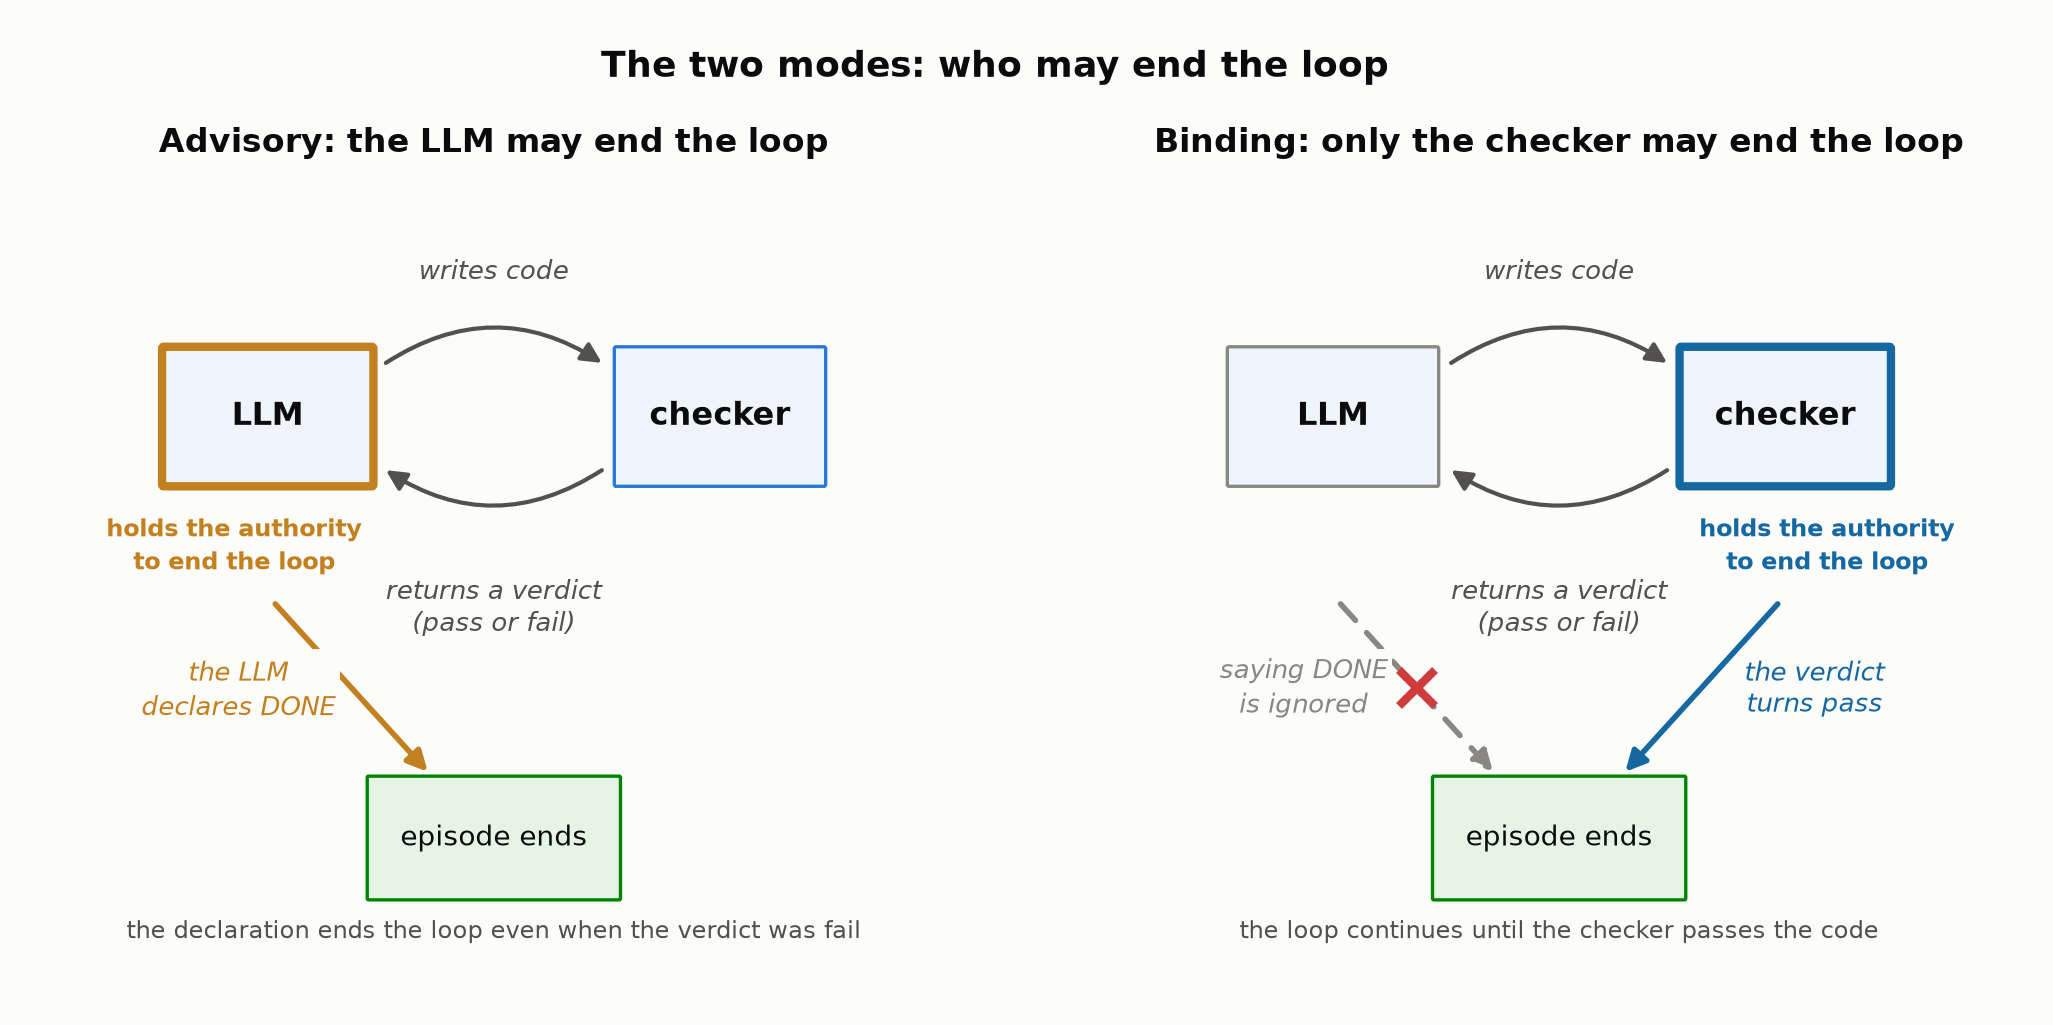
\includegraphics[width=\textwidth]{fig7_modes.png}
\caption{The two modes: the same loop between the LLM and the checker, with the authority to end it held by the LLM in advisory and by the checker in binding. Drawn by \texttt{writeup\_figures/plot\_diagrams.py}.}
\label{fig:modes}
\end{figure}

The failure that separates the two designs is the false-DONE, in which the model submits wrong code and, in the same turn, confidently declares the task finished without waiting for the verdict. This is neither laziness nor defiance of feedback, because the mistake happens earlier than the feedback. Even though the checker is present and available, the model does not wait to consult it. To judge its own work, the model needs the specification that was stripped away, so it fills the gap from its prior knowledge: it has seen thousands of similar functions, so it imposes their learned conventions and constructs the missing specification for itself. It then grades its work against that constructed answer key, finds everything satisfied, and declares done. The answer key is wrong, and the model has no way to know it is wrong, because its only source of task knowledge produced the wrong task. The model does not know when it does not know.

This matters beyond the laboratory because in real deployments the specification is always incomplete. No user writes down every edge case and every convention. An agent is therefore always partly grading itself against a reconstructed answer key, and the question of whether its own ``done'' should carry authority is a design decision every agent system makes, usually without noticing.

\section{Setup}

The corpus is synthetic by design. It consists of 97 tasks generated from 25 hand-written seed functions, where each task is a short, standard-library-only Python function into which exactly one bug has been injected by changing a single line. The bugs are drawn from a closed taxonomy of eight types, such as off-by-one errors, inverted conditions, and deleted edge-case guards. I chose synthetic tasks over organic bugs from real repositories because a synthetic corpus lets me freeze the ground truth. For every task I know the reference solution, the exact error, and the test cases that error is attributed to, so the checker's verdict is authoritative and every failure traces to the one injected bug. In an organic repository the causes of a bug are ambiguous, the correct fix is debatable, and therefore the ground truth itself is debatable. The closed taxonomy has a second benefit: because I know each task's bug class, I can later ask where the failures concentrate, not just how many there are. One honest cost of this choice is that the seed functions are common utilities the models have likely seen in training, which inflates absolute success rates but not the advisory-versus-binding difference the thesis rests on.

The checker runs a submission against the task's frozen test suite in an isolated subprocess and returns a deterministic verdict: PASSED, or FAILED with the names of the failing tests and an error excerpt. The two harnesses share everything that must be shared, including the prompt builder, the verdict renderer, and the checker itself, so the feedback text is byte-identical across arms. They differ in exactly three rules, all on the binding side: completion is computed rather than declared, a byte-identical resubmission after a failure is rejected without re-checking, and three consecutive identical failures end the episode as escalated.

The spec-starved presentation was not the starting point but a logged discovery. Initially the tasks were shown with their full descriptions, and both models solved essentially every dev task in one shot, leaving no difference for the experiment to measure. I then withheld the separate description while leaving the docstrings in the source, and still everything was one-shotted, because the docstrings alone carried enough of the specification. Only after additionally stripping all docstrings and comments from the presented code did the corpus begin to discriminate between the two modes. This presentation was adopted after the pilots but registered before any test-set episode ran.

\begin{figure}[t]
\centering
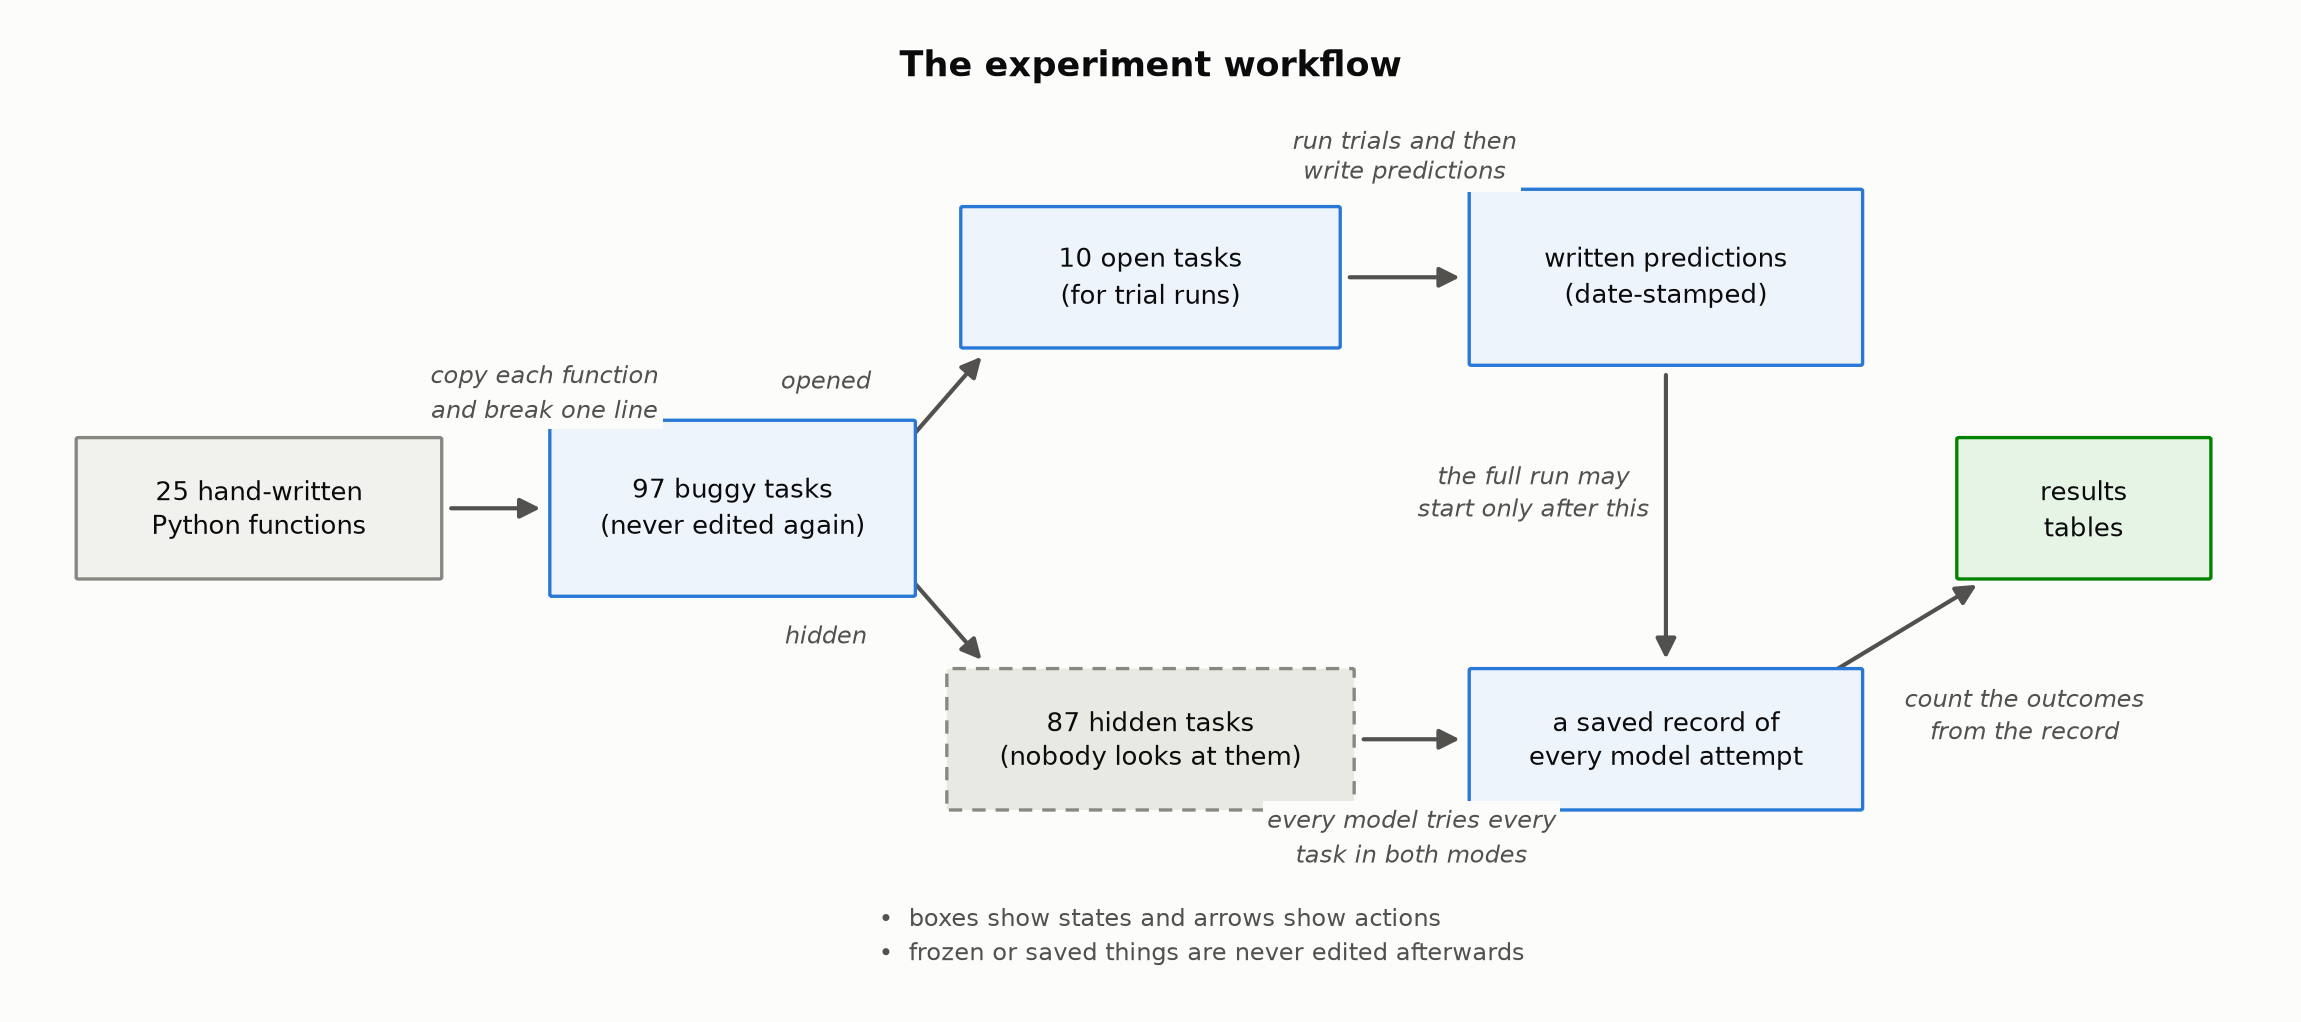
\includegraphics[width=\textwidth]{fig6_workflow.png}
\caption{The experiment workflow: boxes are states and arrows are actions. The hidden test tasks flow to the full run untouched by piloting, and the run may start only after the predictions are locked. Drawn by \texttt{writeup\_figures/plot\_diagrams.py}.}
\label{fig:workflow}
\end{figure}

The discipline around the experiment defends against a single attack: that I fit the experiment to the result. The corpus was frozen with a content hash before the runs, which proves no task was edited after the results existed. Ten tasks were reserved for pilots, and all design decisions, including the presentation changes above, were made while looking only at those ten, so the 87 test tasks stayed unopened until the design was final and cannot have been tuned toward any outcome. The predictions were committed with a git tag before the first paid API call, so the hypotheses provably precede the data. Every deviation from plan was recorded in an append-only log. Both models ran at temperature 0 with a step cap of 8, identical across arms.

\section{Experiment 1: the interaction}

\paragraph{Results:} The rows of the table are the two models, weak (gpt-4o-mini) and strong (gpt-4.1), and the columns are the two modes, with each cell showing the number of tasks solved out of 87.

\begin{table}[h]
\centering
\begin{tabular}{lccc}
\toprule
 & advisory & binding & $\Delta$ (binding $-$ advisory)\\
\midrule
weak (gpt-4o-mini) & 79/87 (90.8\%) & 87/87 (100\%) & +9.2 pp\\
strong (gpt-4.1) & 87/87 (100\%) & 87/87 (100\%) & +0.0 pp\\
\bottomrule
\end{tabular}
\caption{Experiment 1 success rates. Source: \texttt{phase6\_analysis/results.md}, regenerated deterministically from the committed logs.}
\label{tab:exp1}
\end{table}

\paragraph{Reading the table:} Three of the four cells sit at 100\%, so the experiment effectively lives in the weak-advisory cell, which loses 8 tasks. Since the effect of mode clearly depends on which model it is applied to, the two factors are coupled, and the correct summary of the table is their interaction rather than either factor alone.

\paragraph{Interaction term:} It is defined as the difference of differences, which here is 9.2 $-$ 0.0 = +9.2 percentage points. Binding helps the weak model, and does nothing measurable for the strong one.

\paragraph{Statistical test:}

\emph{Definition:} Both arms ran the same 87 tasks, so each task has a pair of outcomes, one from advisory and one from binding. A task where both modes succeed, or both fail, tells us nothing about the difference between the modes, so the test uses only the tasks where the two modes disagree. There are two directions of disagreement: b is the count of tasks solved in advisory but failed in binding, and c is the count of tasks solved in binding but failed in advisory. The null hypothesis is that mode has no effect on outcomes. If that is true, then each disagreement is equally likely to fall in either direction, with probability one half, and the probability of observing a split as extreme as (b, c) is given by the exact binomial distribution. This is the McNemar test.

\emph{Calculation:} For the weak model, the observed split is b = 0 and c = 8, and the probability of all eight disagreements falling on one side of a fair coin is p = 2 $\times$ $(1/2)^8$ = 0.0078. For the strong model, b = 0 and c = 0, so there are no disagreements and no test to run.

\emph{Inference:} The p-value of 0.0078 rejects the null hypothesis for the weak model, so the mode difference is statistically real and not a chance pattern across 8 tasks. The value b = 0 adds a separate fact: binding never lost a single task that advisory had solved, so the improvement came without any losses. For the strong model, the absence of disagreements means the two modes were behaviorally identical.

\begin{figure}[t]
\centering
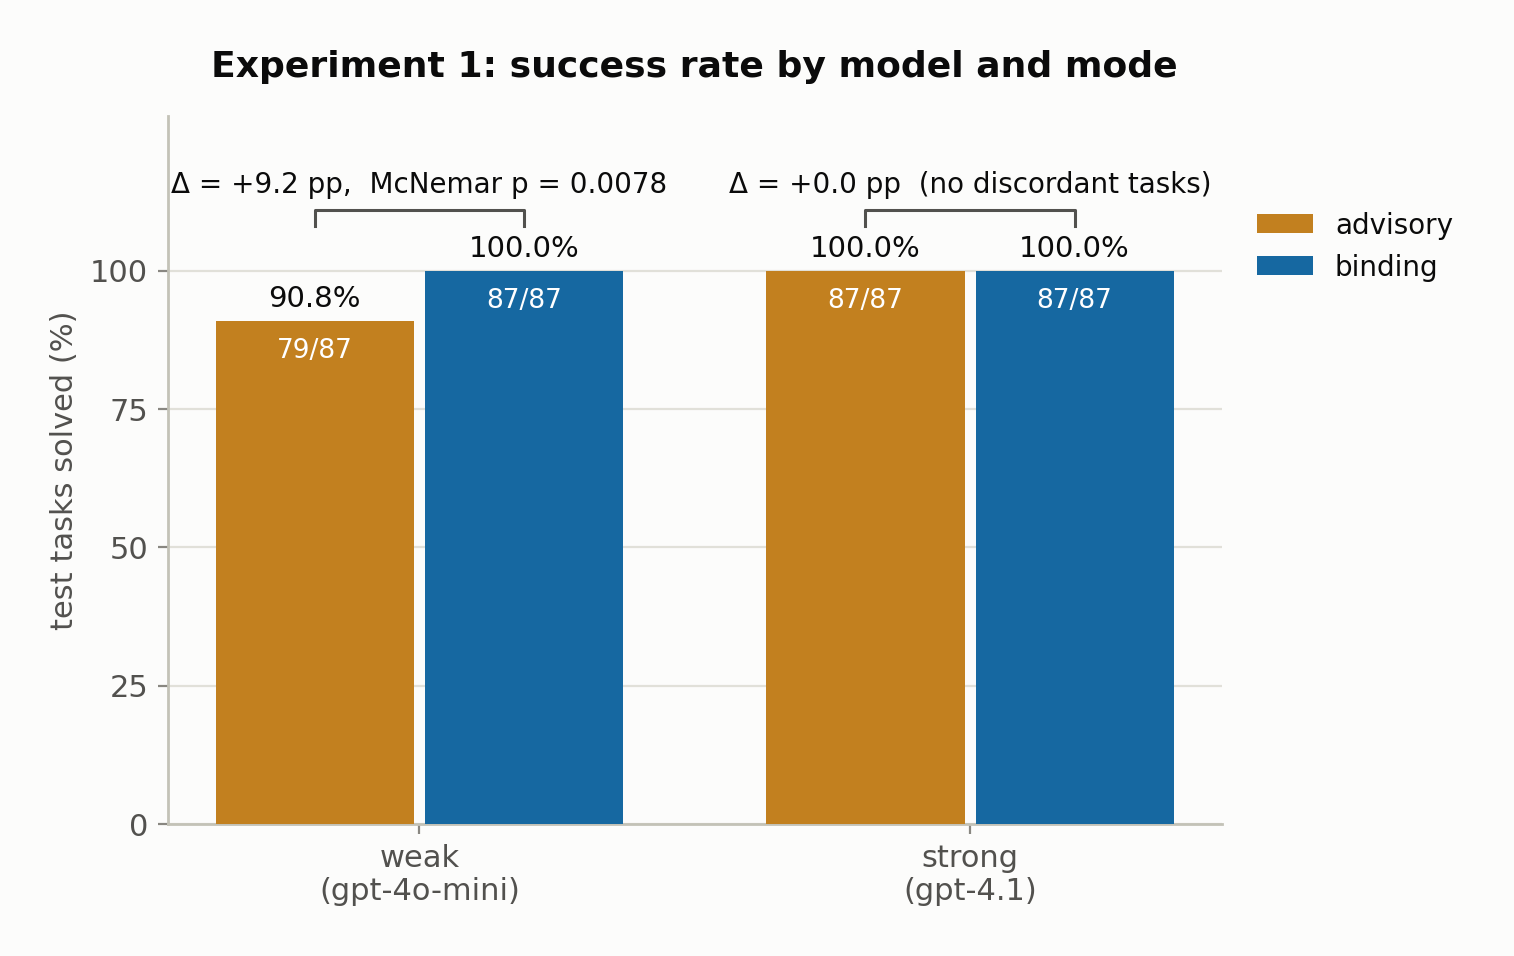
\includegraphics[width=0.85\textwidth]{fig1_experiment1_2x2.png}
\caption{Experiment 1 success rate by model and mode. Drawn by \texttt{writeup\_figures/plot\_all.py} from \texttt{writeup\_figures/data/exp1\_results.csv}.}
\label{fig:exp1}
\end{figure}

\paragraph{Failure breakdown:} When the weak-advisory cell is broken down by bug type, a single class accounts for 6 of the 8 failures: missing-edge-case bugs, solved 9/15 in advisory against 15/15 in binding. This class deletes a guard whose requirement was documented only in the docstring that the presentation strips, so the failures concentrate exactly where the withheld specification mattered most.

\paragraph{Interpreting the failures:} A reviewer may object that a corpus the weak model fully solves under binding must be too easy to be informative. The objection misses what the ceiling establishes: binding at 100\% demonstrates that every task was within the model's ability to solve under this harness, so the 8 advisory failures were not tasks the model could not do, they were tasks on which it quit while wrong. On a harder corpus, failures of ability and failures of judgment would mix together, and no later analysis could separate them, which is why the easy corpus works as an isolation mechanism rather than a weakness.

\paragraph{Breakdown of the rescues:} The 8 rescues are not all of one kind. In 6 of them binding produced a genuine forced repair, meaning a FAILED verdict followed by a changed submission that passed. In the remaining 2, binding's first submission happened to pass while advisory's first draft on the same task false-DONEd, which is sampling variance at temperature 0 rather than iteration. The +9.2 pp therefore carries a small stochastic component, and it is reported rather than rounded away.

\paragraph{The strong model:} The strong model was not spared failing verdicts, as it hit FAILED mid-episode on 6 tasks in advisory. It then iterated to a passing solution before declaring done in every case, averaging 2.02 steps per task against the weak model's 1.20. A model that already waits for green before claiming leaves binding nothing to catch.

\paragraph{Contribution of the three rules:} Binding consists of three rules, but identical-resubmission rejection and escalation never fired across all 348 episodes. The entire effect therefore comes from computed completion alone, the rule that the model may not quit while the checker is red.

\paragraph{Cost:} For the strong model, binding was also 31\% cheaper, \$0.107 against \$0.155, because binding ends the moment the checker passes while advisory spends additional tokens composing its declaration. The same cost pattern reappears in both later experiments.

\section{Experiment 2: the capability ladder}

\paragraph{Bridge from Experiment 1:} Experiment 1 produced a 2×2 table, which for the capability question is just two points: a weak model helped by +9.2 pp and a strong model unchanged. Two points can always be connected by a line, and the line suggested here is a tempting one: the weaker the model, the larger the binding advantage. If that line were real, binding would be a general safety net, and the frailer the model the more one would gain by bolting it on. Experiment 2 was built to test the line. The design follows directly: keep the dataset and every harness condition exactly as they were, pass multiple models of graded capability through the same tasks, and place each model's $\Delta$ = success(binding) $-$ success(advisory) on a capability axis. The registered expectation was monotone: $\Delta$ should only rise as capability falls.

\paragraph{Preconditions:} Experiment 2 runs seven models: Llama-3.2-3B, Llama-3.1-8B, Qwen2.5-7B, Claude-3-Haiku, GPT-4o-mini, Gemini-2.5-Flash-Lite, and GPT-4.1, of which the last two are carried over from Experiment 1 as anchors, and each is pinned to an exact snapshot ID. No other condition changes. The corpus, the dev-test split, the bare-code presentation, the prompts, the harness rules, the checker, temperature 0, and step cap 8 are all inherited from Experiment 1 and hash-verified before the run. The scale follows from the design: 7 models × 2 modes × 87 test tasks = 1,218 episodes, all committed with zero errors. Because everything except the model is held fixed, any change in $\Delta$ across the ladder is attributable to capability alone.

\paragraph{The capability ranking:} The seven models must be placed on a capability axis before the experiment runs. The ranking uses two published sources, snapshotted on a fixed date before any episode: the LMArena Chatbot Arena Elo score and the MMLU (5-shot) score reported on each vendor's official model card. The combining rule is fixed and mechanical. Within each source, models are ranked 1 for the strongest upward in order of that source's score. Each model's composite score is the mean of its per-source ranks, and a model absent from a source is ranked only on the sources that list it, which applies to Qwen2.5-7B since it was absent from the Elo snapshot. The ladder is ordered by ascending composite score, and any tie would be broken by the Elo rank. No tie arose.

The resulting order, from strongest to weakest:

1. GPT-4.1\\
2. Gemini-2.5-Flash-Lite\\
3. GPT-4o-mini\\
4. Claude-3-Haiku\\
5. Qwen2.5-7B\\
6. Llama-3.1-8B\\
7. Llama-3.2-3B

The ranking was computed this way for one reason. The experiment plots $\Delta$ against capability, so capability must be measured independently of the experiment's own data. If the models were ranked by their success on our tasks, the curve would be our data plotted against itself. Using external published benchmarks, combined by a rule stated in advance and locked with a git tag before the first episode, makes the x-axis independent of everything the experiment later measures.

\paragraph{Predictions:} Five predictions were registered and locked before the first episode. The first four are confirmatory and the fifth is explicitly exploratory.

1. $\Delta \geq 0$ for every model, meaning binding never hurts.\\
2. $\Delta$ decreases with capability, tested as a one-sided Spearman correlation against the fixed ranking.\\
3. The advisory false-DONE rate decreases with capability.\\
4. For any model at the advisory ceiling, binding total cost is at most advisory total cost.\\
5. Exploratory: $\Delta$ may reverse at the weak end, because a model can be too weak to rescue. If observed, this defines a capability window for completion gating.

\paragraph{Results:} The main table has one row per model, ordered strongest to weakest by the locked ranking, with each cell showing tasks solved out of 87. The columns b and c are the paired disagreement counts defined in Experiment 1, and p is the exact McNemar value.

\begin{table}[h]
\centering
\begin{tabular}{clcccccc}
\toprule
rank & model & advisory & binding & $\Delta$ (pp) & b & c & exact p\\
\midrule
1 & GPT-4.1 & 87/87 & 87/87 & +0.0 & 0 & 0 & 1\\
2 & Gemini-2.5-Flash-Lite & 79/87 & 87/87 & +9.2 & 0 & 8 & 0.0078\\
3 & GPT-4o-mini & 79/87 & 87/87 & +9.2 & 0 & 8 & 0.0078\\
4 & Claude-3-Haiku & 72/87 & 82/87 & +11.5 & 2 & 12 & 0.013\\
5 & Qwen2.5-7B & 71/87 & 84/87 & +14.9 & 0 & 13 & 0.00024\\
6 & Llama-3.1-8B & 80/87 & 82/87 & +2.3 & 3 & 5 & 0.73\\
7 & Llama-3.2-3B & 66/87 & 63/87 & $-$3.4 & 9 & 6 & 0.61\\
\bottomrule
\end{tabular}
\caption{The ladder. Source: \texttt{v2\_ladder/analysis/results.md}, regenerated from the committed logs.}
\label{tab:ladder}
\end{table}

\begin{figure}[H]
\centering
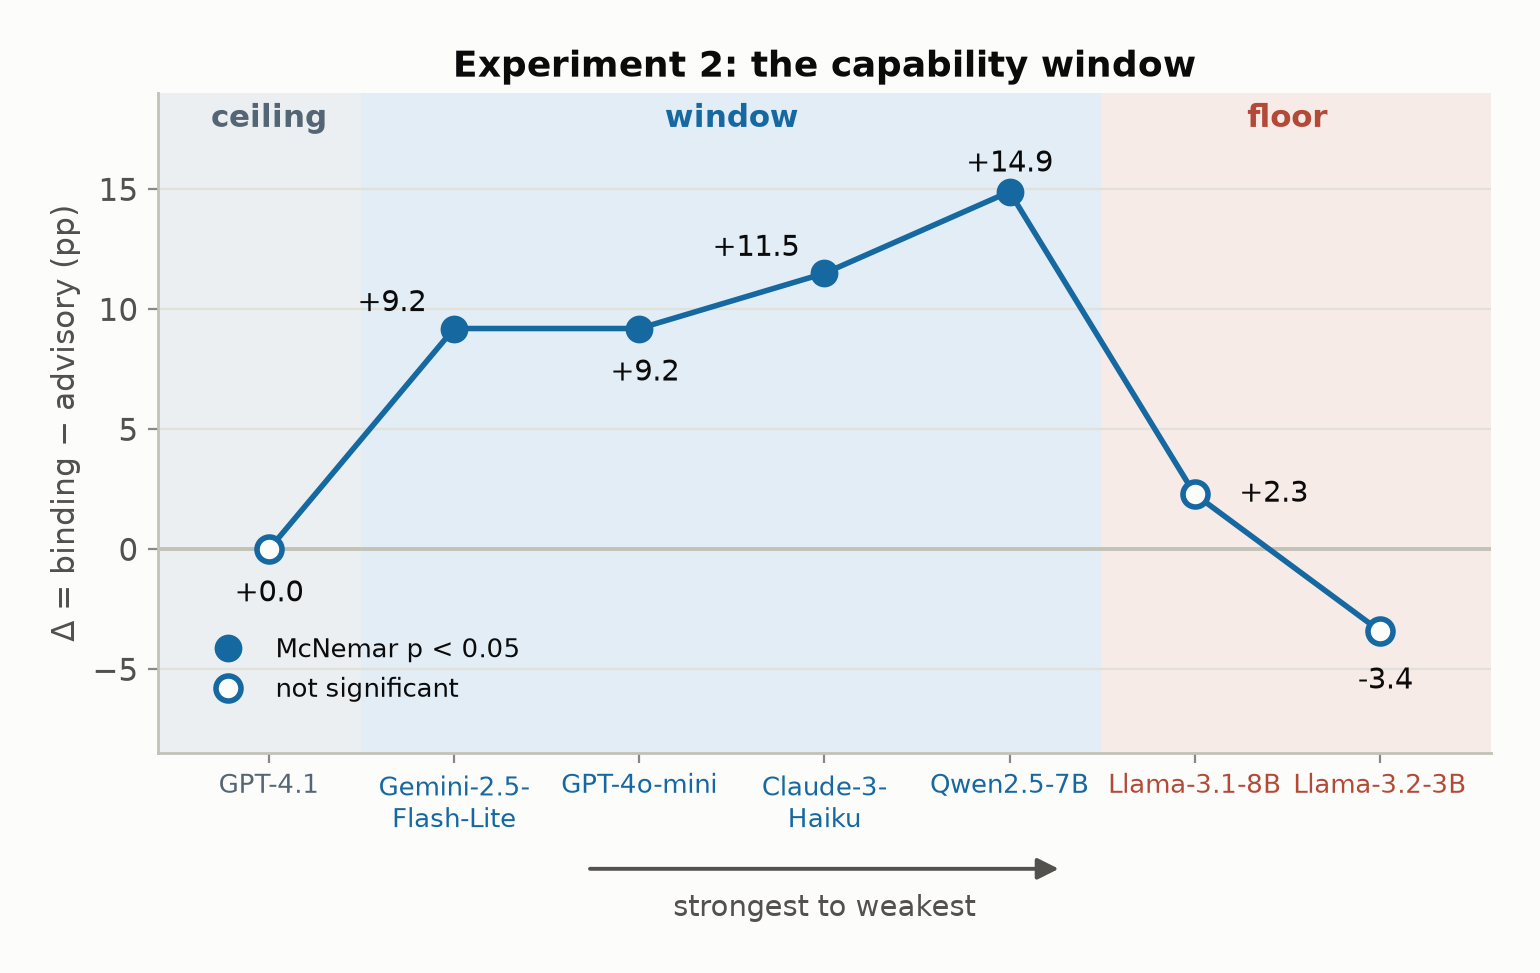
\includegraphics[width=\textwidth]{fig2_capability_window.png}
\caption{The capability window: the three regimes as shaded bands, filled dots for McNemar-significant rungs. Drawn by \texttt{writeup\_figures/plot\_all.py} from \texttt{writeup\_figures/data/exp2\_ladder.csv}.}
\label{fig:window}
\end{figure}

\paragraph{Reading the curve:} The registered expectation was that $\Delta$ rises steadily as models weaken. The observed curve does something else. $\Delta$ starts at zero for the strongest model, rises through the middle of the ladder, peaks at Qwen2.5-7B with +14.9, then collapses at the weak end and crosses below zero at the weakest rung, where binding makes the model worse by 3.4 points. The shape is a window with a ceiling and a floor, not a slope.

\paragraph{Statistical test:}

\emph{Definition:} Prediction 2 claims a monotone relation between $\Delta$ and capability rank. The Spearman rank correlation measures exactly this: it is +1 when $\Delta$ only rises as rank weakens, $-$1 when $\Delta$ only falls, and near 0 when there is no consistent direction. The test is one-sided in the registered direction, and the p-value is exact, computed by comparing the observed correlation against all 5,040 possible orderings of 7 ranks.

\emph{Calculation:} The observed correlation is rho = $-$0.13 with p = 0.62.

\emph{Inference:} The prediction is not confirmed, and the correlation is slightly negative, which is the wrong sign. The cause is visible in the results table: the trend holds from rank 1 to rank 5 and then reverses at ranks 6 and 7, so the weak end breaks the monotone story. Per rung, the McNemar values show the middle of the ladder is individually significant, with p from 0.013 down to 0.00024, while neither weak rung is.

\paragraph{Scoring the predictions:} Prediction 1 is disconfirmed, since $\Delta$ is negative at the weakest rung. Prediction 2 is disconfirmed by the Spearman test above. Prediction 3 is disconfirmed, since the false-DONE counts form a hump rather than a slope, as shown below. Prediction 4 is confirmed at the one rung where it can be tested, since GPT-4.1 is the only model at advisory ceiling. Prediction 5, the exploratory one, is observed, and it names the finding: a capability window. Three of four confirmatory predictions failed, and reporting them as failures rather than adjusting them afterwards is what the preregistration was for.

\paragraph{Exit classification:} Every episode ends at exactly one exit. Advisory has four end states: the model declares done and the code passes (true-DONE), the model declares done and the code fails (false-DONE), the step cap is reached with passing code the model never recognized (cap, code passing), and the step cap is reached with failing code (cap, code failing). Binding has three: the checker passes (solved), three identical failed submissions (escalated), and the step budget runs out (step cap). Each mode's columns sum to 87.

\begin{figure}[H]
\centering
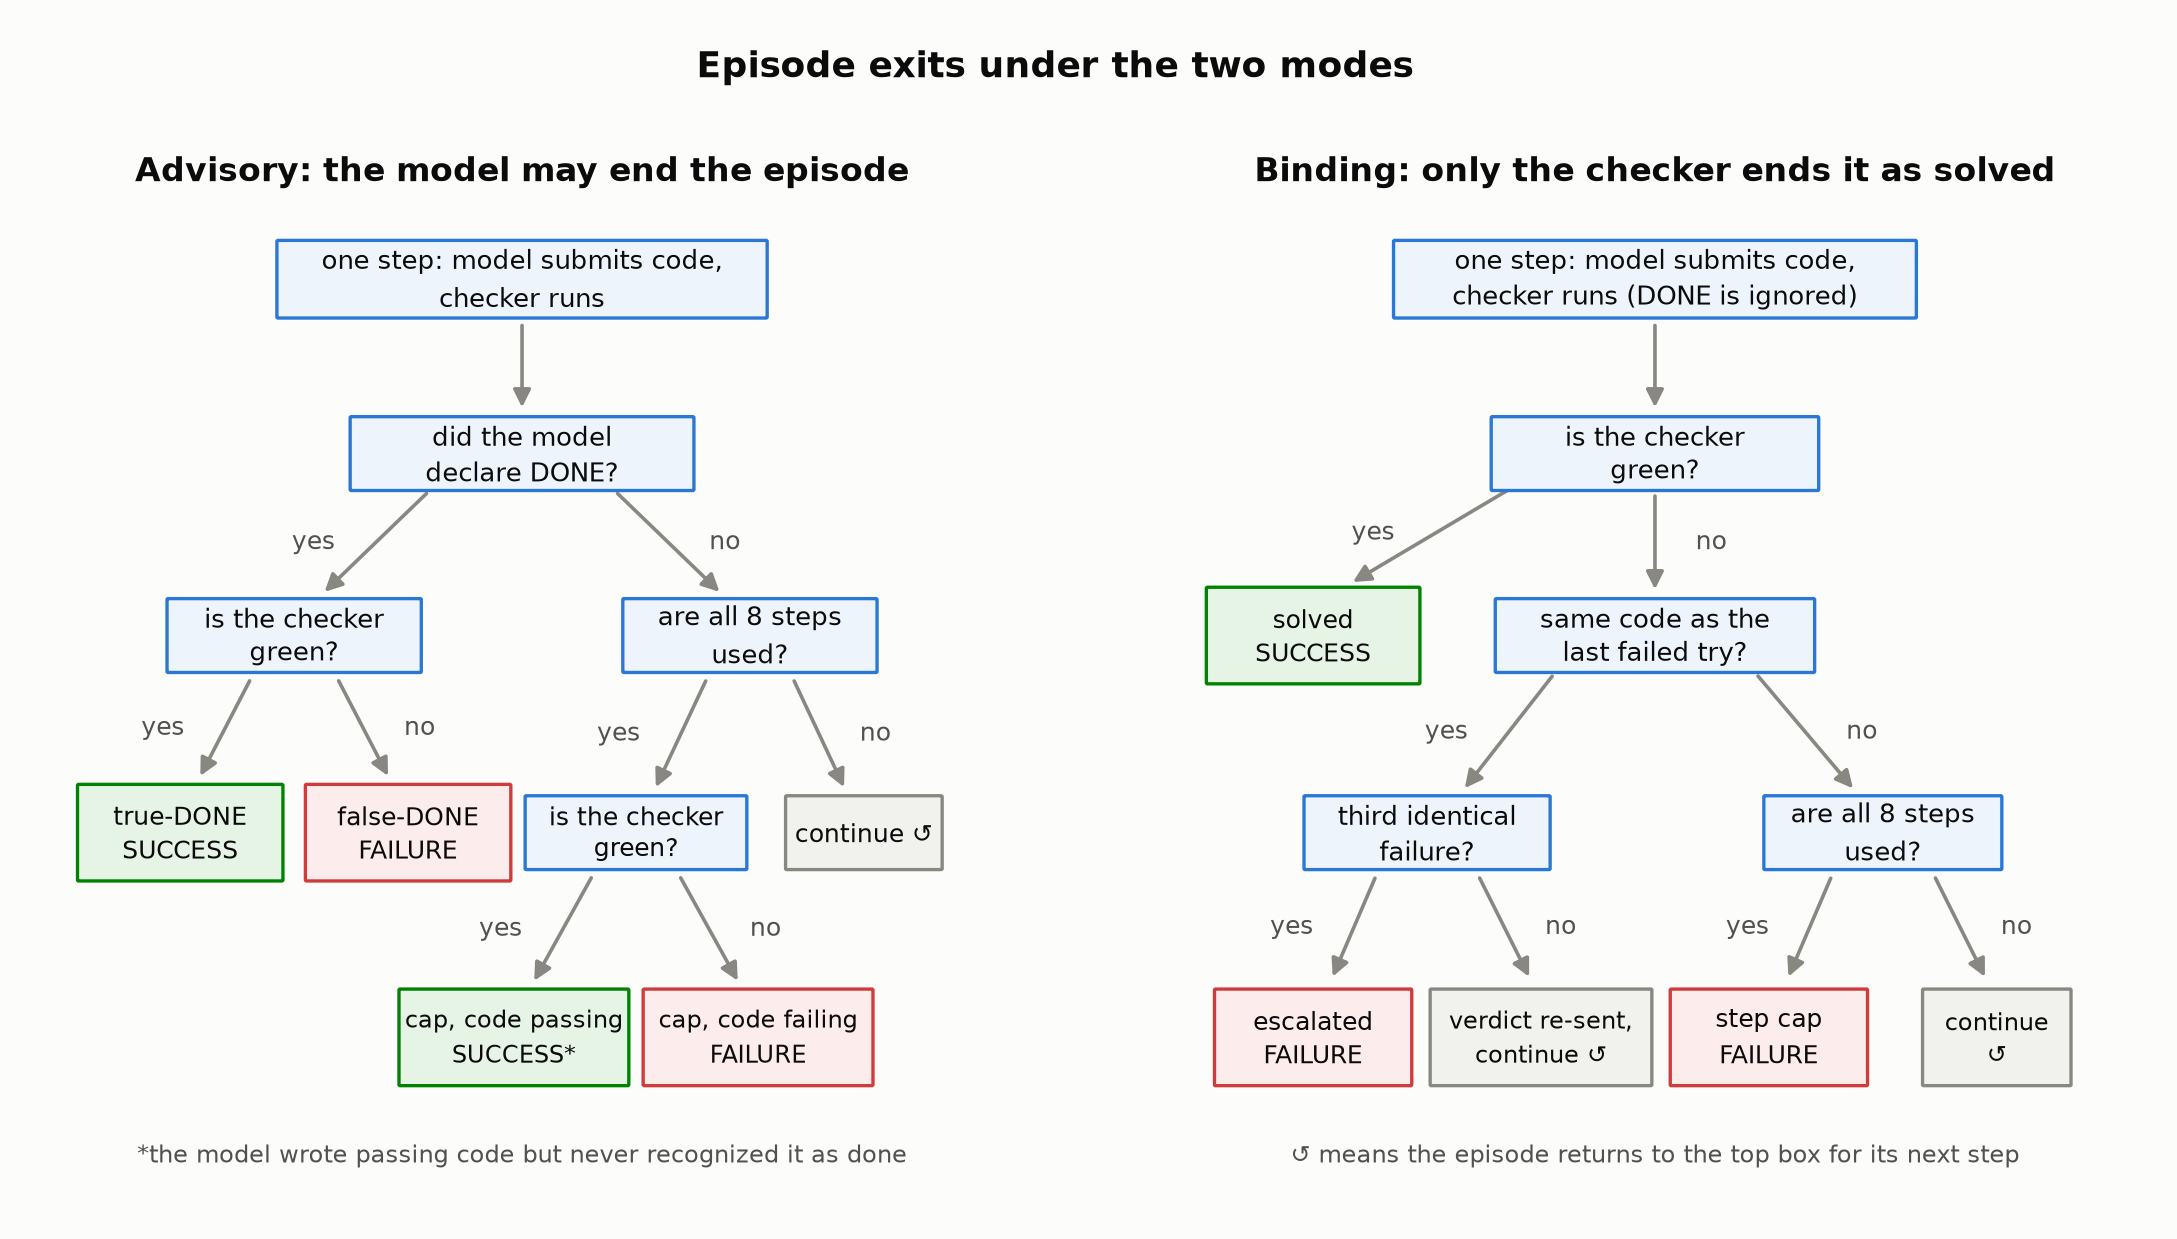
\includegraphics[width=\textwidth]{fig5_exit_trees.png}
\caption{Episode exits under the two modes, as decision trees. Drawn by \texttt{writeup\_figures/plot\_diagrams.py}.}
\label{fig:exits}
\end{figure}

\begin{table}[H]
\centering
\small
\setlength{\tabcolsep}{4.5pt}
\begin{tabular}{lcccccccc}
\toprule
 & \multicolumn{4}{c}{advisory} & \multicolumn{3}{c}{binding} & \\
\cmidrule(lr){2-5}\cmidrule(lr){6-8}
model & true-DONE & false-DONE & cap pass & cap fail & solved & escalated & step cap & $\Delta$ (pp)\\
\midrule
GPT-4.1 & 87 & 0 & 0 & 0 & 87 & 0 & 0 & +0.0\\
Gemini-2.5-Flash-Lite & 79 & 8 & 0 & 0 & 87 & 0 & 0 & +9.2\\
GPT-4o-mini & 79 & 8 & 0 & 0 & 87 & 0 & 0 & +9.2\\
Claude-3-Haiku & 72 & 15 & 0 & 0 & 82 & 4 & 1 & +11.5\\
Qwen2.5-7B & 71 & 16 & 0 & 0 & 84 & 3 & 0 & +14.9\\
Llama-3.1-8B & 80 & 4 & 0 & 3 & 82 & 2 & 3 & +2.3\\
Llama-3.2-3B & 56 & 1 & 10 & 20 & 63 & 10 & 14 & $-$3.4\\
\bottomrule
\end{tabular}
\caption{Exit classification: every episode falls into exactly one column, and each mode's columns sum to 87 per model. Source: \texttt{v2\_ladder/analysis/results.json}.}
\label{tab:exits}
\end{table}

\paragraph{Patterns in the table:} Reading each column down the ladder, from strongest model to weakest, three number series form the section's findings.

The false-DONE series is 0, 8, 8, 15, 16, 4, 1. The pattern is a hump: false claiming is absent at the top, frequent in the middle, and nearly absent again at the bottom. The inference is that confident wrong completion is a mid-capability phenomenon, since it requires enough capability to construct a plausible answer and claim it, which the weakest models do not reach.

The $\Delta$ series is +0.0, +9.2, +9.2, +11.5, +14.9, +2.3, $-$3.4. The pattern is a window: zero at the top, rising to a peak in the middle, then collapsing below zero at the bottom. The inference is that the binding advantage tracks the false-DONE hump almost exactly, because binding creates value only by converting false claims into forced repairs, so where there are no false claims there is nothing to convert.

The advisory step cap series, taking both cap columns together, is 0, 0, 0, 0, 0, 3, 30. The pattern is a floor signature: step capping appears only at the weak end and explodes at the weakest rung. The inference is that the weakest model fails by thrashing rather than by false claiming, including 10 episodes where it had already written passing code and did not recognize it, and for a thrashing model binding's forced iteration adds failure exits instead of rescues.

\paragraph{The floor:} The weakest model is the one binding hurts, and the mechanism is visible in its exits. Binding lost 9 tasks that advisory had solved: 5 ended escalated after three identical failed submissions and 4 burned all eight steps still failing. Forced iteration helps a model whose next attempt can be better, but for a model that thrashes, extra forced turns are extra chances to trip the harness machinery. Two binding rules that stayed dormant through all of Experiment 1 came alive at the weak end here: identical-resubmission rejection fired 37 times for Llama-3.2-3B, and escalation ended 10 of its episodes. The statement from Experiment 1 that only computed completion ever fires is therefore true of Experiment 1 only, and the first recorded contribution of the other two rules was harm.

\paragraph{The window interior:} The models in the middle of the ladder share a specific profile: capable enough to produce a plausible wrong answer and declare it done, and capable enough to repair once the claim is refused. Both halves are visible in the logs. Qwen's 13 rescues contain 12 genuine forced repairs, meaning a FAILED verdict followed by a changed submission that passed, and Haiku's 12 contain 10, so the middle of the ladder is rescued by real iteration rather than sampling luck. The rescued tasks concentrate again in missing-edge-case bugs, 8 of Qwen's 13 and 6 of Haiku's 12, the same specification-carrying class as Experiment 1.

\paragraph{Replication:} GPT-4o-mini reproduces its Experiment 1 result exactly, +9.2 with b = 0 and c = 8, and GPT-4.1 reproduces its zero. Gemini-2.5-Flash-Lite, from a different provider, lands on the same +9.2 with the same split.

\paragraph{Cost:} Prediction 4 holds at the ceiling: GPT-4.1 under binding cost \$0.104 against \$0.157 under advisory, cheaper by a third, for the same structural reason as in Experiment 1. One economic observation follows: Qwen2.5-7B under binding reaches 84/87, three tasks short of GPT-4.1, at roughly 2\% of GPT-4.1's advisory cost.

\paragraph{Deviations:} Two of the 14 cells stalled mid-run on slow provider connections and were re-run to completion under a hard per-episode deadline. The interruption is recorded as a logged deviation, and all 1,218 episode logs are schema-identical.

\paragraph{Inference:} The line drawn from Experiment 1 is dead. Binding is not a safety net that pays more the weaker the model. It pays inside a window: below the ceiling, because a model at ceiling never false-claims, and above the floor, because a model that cannot iterate on feedback is not rescued by being forced to iterate. The value of the gate tracks the false-DONE rate, and false claiming is a mid-capability phenomenon. This raises the question Experiment 3 exists to answer: is the window a property of the model, or of the model and task together? If task difficulty rises, does the window slide up the capability axis?

\section{Experiment 3: the composition window}

\paragraph{Bridge from Experiment 2.} Experiment 2 replaced the line with a window: binding pays off in a middle band of capability, does nothing at the ceiling, and hurts below the floor. But the ladder varied only the model, holding task difficulty fixed at one bug per task, so the window it drew is a slice at a single difficulty. This leaves the sharpest question of the program open: is the window a property of the model, or of the model and task together? The two hypotheses make different predictions. If the window belongs to the model--task pair, then difficulty and capability trade off, and raising the difficulty should make the window slide up the capability axis, so that a model at the ceiling begins to false-claim and binding begins to help it. If the window belongs to the model alone, the ceiling stays where it is no matter how hard the task becomes. Experiment 3 was built to decide between the two. The design follows directly: keep the models and every harness condition exactly as they were, turn the other knob by raising task difficulty in controlled steps, and measure each model's $\Delta$ at every difficulty tier. The registered expectation was that the window slides: by the hardest tier, the strongest model's false-DONE count becomes positive and its $\Delta$ turns positive with it.

\paragraph{Preconditions.} Experiment 3 changes exactly one factor: task difficulty. Difficulty is raised by bug composition, where a k1 task applies 2 of the original Experiment 1 mutations verbatim on distinct lines of one seed function, and a k2 task applies 3. Nothing new is authored, since the generator only selects and composes the frozen v1 mutations, so a harder task means more independent bugs at once and nothing else. The two tiers are frozen with their own content hashes and dev-test splits: 60 test tasks at k1 and 48 at k2, with 10 dev tasks per tier used only for calibration.

The roster is six models spanning the Experiment 2 ladder: Llama-3.1-8B as the bottom-edge anchor, the four window models Qwen2.5-7B, Claude-3-Haiku, GPT-4o-mini, and Gemini-2.5-Flash-Lite, and GPT-4.1 as the top anchor. Llama-3.2-3B is dropped, as a logged roster decision: it was already below the window at one bug per task, failing by step cap rather than false claim, so raising difficulty could only push it further out of range and buy noise instead of signal.

No other condition changes. The harnesses, the three binding rules, the bare-code presentation, the checker, temperature 0, step cap 8, and each model's exact snapshot and route are inherited from the earlier experiments unchanged. The k0 column of every result is Experiment 2's committed test data, cited from its manifests rather than re-run, which keeps the baseline comparable and spends nothing. The scale follows from the design: 6 models × 2 modes × 108 test tasks = 1,296 episodes, all committed with zero errors.

Because everything except difficulty is held fixed, any change in a model's $\Delta$ across the tiers is attributable to task difficulty alone.

\paragraph{Predictions.} Five predictions were registered and locked with a git tag before any test episode ran. One disclosure inside the registration matters for reading them: before registering, a small calibration was run on 10 dev tasks per tier and its results were quoted verbatim in the preregistration itself. That glimpse showed GPT-4.1 with zero false-DONEs at both tiers. Prediction 2 was registered against that glimpse deliberately, on the reasoning that 10 tasks cannot surface a low-rate event that theory expected to appear on the larger sealed test sets. This makes it a risky prediction rather than a restatement of what the dev data already showed.

1. For each window model, $\Delta$ > 0 at both k1 and k2, by per-model task-paired exact McNemar.\\
2. The window is a property of the model--task pair: as difficulty rises, models above the window enter the false-claiming regime. Operationally, GPT-4.1's advisory false-DONE count, zero at one bug per task, becomes positive at k2, and its $\Delta$ turns positive with it.\\
3. Escalation-attributed losses, meaning tasks solved in advisory but lost in binding through escalation, concentrate at the bottom-edge anchor and grow with k. The escalation rule is deliberately left unchanged so that this known wart becomes a measured quantity.\\
4. For any model at the advisory ceiling within a tier, binding total cost is at most advisory total cost.\\
5. Exploratory: the window peak, the model with the largest $\Delta$, shifts toward stronger models as k rises.

\paragraph{Results.} The central table is the $\Delta$-vs-k matrix, one row per model, showing $\Delta$ = success(binding) $-$ success(advisory) in percentage points at each difficulty tier. The k0 column is Experiment 2's committed test data.

\begin{table}[h]
\centering
\begin{tabular}{lccc}
\toprule
model & $\Delta$ @ k0 (1 bug) & $\Delta$ @ k1 (2 bugs) & $\Delta$ @ k2 (3 bugs)\\
\midrule
GPT-4.1 & +0.0 & +0.0 & +0.0\\
Gemini-2.5-Flash-Lite & +9.2 & +23.3 & +22.9\\
GPT-4o-mini & +9.2 & +23.3 & +22.9\\
Claude-3-Haiku & +11.5 & +26.7 & +25.0\\
Qwen2.5-7B & +14.9 & +31.7 & +22.9\\
Llama-3.1-8B & +2.3 & +10.0 & +2.1\\
\bottomrule
\end{tabular}
\caption{The $\Delta$-vs-k matrix. Source: \texttt{v3\_window/analysis/results.md}, with the k0 column cited from Experiment 2.}
\label{tab:matrix}
\end{table}

The full per-cell results behind the matrix, with the paired disagreement counts and exact McNemar values:

\begin{table}[h]
\centering
\begin{tabular}{llcccccc}
\toprule
model & tier & advisory & binding & $\Delta$ (pp) & b & c & exact p\\
\midrule
Llama-3.1-8B & k1 & 49/60 & 55/60 & +10.0 & 1 & 7 & 0.070\\
Llama-3.1-8B & k2 & 42/48 & 43/48 & +2.1 & 3 & 4 & 1\\
Qwen2.5-7B & k1 & 36/60 & 55/60 & +31.7 & 0 & 19 & 3.8e-06\\
Qwen2.5-7B & k2 & 32/48 & 43/48 & +22.9 & 1 & 12 & 0.0034\\
Claude-3-Haiku & k1 & 41/60 & 57/60 & +26.7 & 2 & 18 & 0.0004\\
Claude-3-Haiku & k2 & 33/48 & 45/48 & +25.0 & 0 & 12 & 0.0005\\
GPT-4o-mini & k1 & 46/60 & 60/60 & +23.3 & 0 & 14 & 0.0001\\
GPT-4o-mini & k2 & 37/48 & 48/48 & +22.9 & 0 & 11 & 0.001\\
Gemini-2.5-Flash-Lite & k1 & 46/60 & 60/60 & +23.3 & 0 & 14 & 0.0001\\
Gemini-2.5-Flash-Lite & k2 & 37/48 & 48/48 & +22.9 & 0 & 11 & 0.001\\
GPT-4.1 & k1 & 60/60 & 60/60 & +0.0 & 0 & 0 & 1\\
GPT-4.1 & k2 & 48/48 & 48/48 & +0.0 & 0 & 0 & 1\\
\bottomrule
\end{tabular}
\caption{Per model and tier results. Source: \texttt{v3\_window/analysis/results.md}.}
\label{tab:cells}
\end{table}

\begin{figure}[t]
\centering
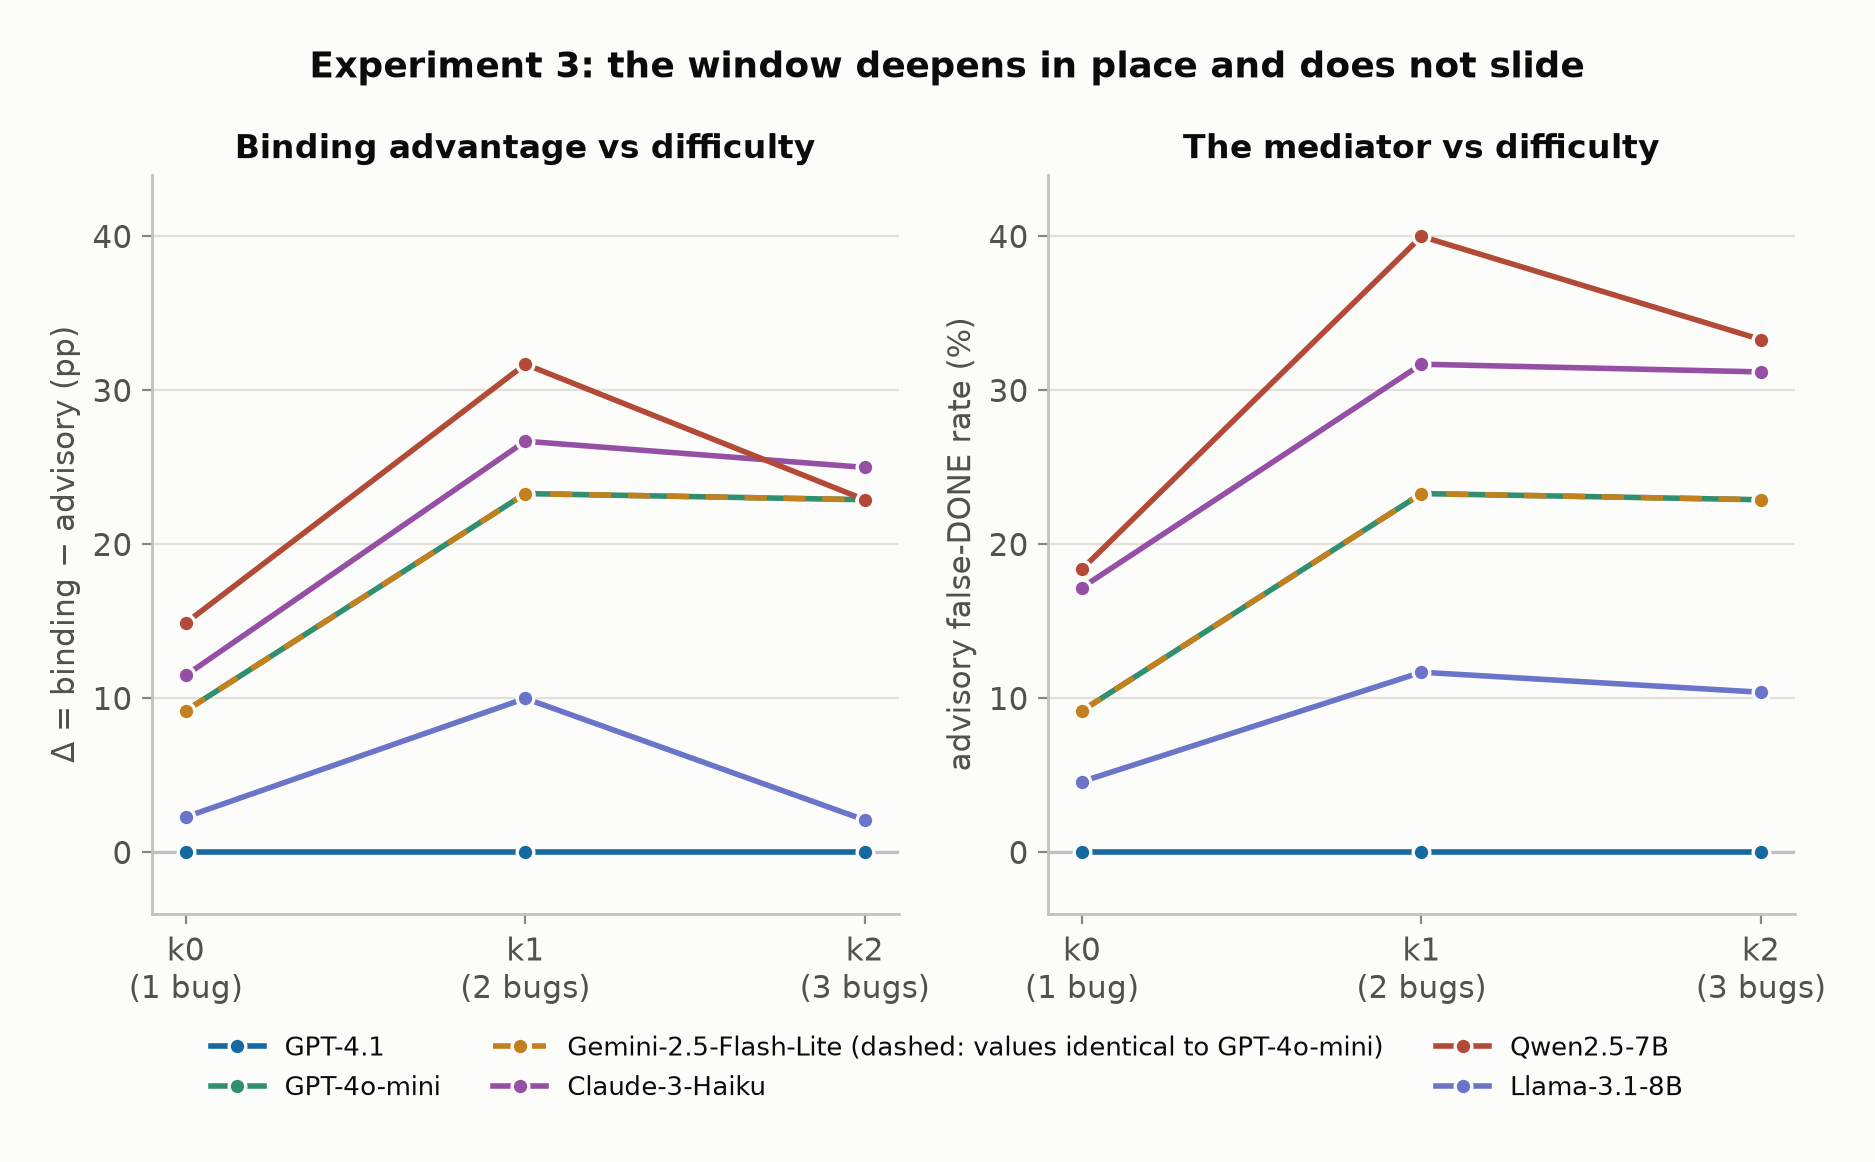
\includegraphics[width=\textwidth]{fig3_composition_window.png}
\caption{The window deepens in place and does not slide: the binding advantage on the left, the advisory false-DONE rate on the right, with the same shape in both panels. Drawn by \texttt{writeup\_figures/plot\_all.py} from \texttt{writeup\_figures/data/exp3\_matrix.csv}.}
\label{fig:composition}
\end{figure}

\paragraph{Reading the matrix.} Two things happen at once, and only one of them was predicted. Reading the window rows left to right, every window model's $\Delta$ roughly doubles from k0 to k1 and stays large at k2, with every window cell McNemar-significant. The window deepens as bugs compose. Reading the GPT-4.1 row, nothing happens at all: 60/60 and 48/48 in both modes, zero disagreements, $\Delta$ pinned at exactly zero at every tier. A difficulty at which Qwen false-claims 40\% of the time did not extract a single false claim from the strongest model. The window deepened in place, and it did not slide.

\paragraph{Patterns in the table.} Reading the matrix by rows and columns, three number series form the section's findings.

The GPT-4.1 row is +0.0, +0.0, +0.0, with false-DONE counts 0, 0, 0. The pattern is a fixed ceiling. The inference is that the window's upper edge did not move under difficulty, which is the disconfirmation of prediction 2 and the headline of the experiment.

The Qwen row is +14.9, +31.7, +22.9. The pattern is deepen-then-plateau, and every window row shows it: the gain roughly doubles at k1 and dips slightly at k2. The inference is that composition amplifies binding for models already inside the window, but the amplification saturates rather than growing without bound.

The Llama-3.1-8B row is +2.3, +10.0, +2.1. The pattern is an edge model sliding toward the floor: its gain rises at k1, then collapses at k2 as it begins to fail by thrashing rather than false claiming. The inference is that difficulty does move the window's floor, just never its ceiling.

\paragraph{The mediator.} The advisory false-DONE rate per model per tier, k0 $\rightarrow$ k1 $\rightarrow$ k2: Qwen 18\% $\rightarrow$ 40\% $\rightarrow$ 33\%, Haiku 17\% $\rightarrow$ 32\% $\rightarrow$ 31\%, GPT-4o-mini and Gemini both 9\% $\rightarrow$ 23\% $\rightarrow$ 23\%, Llama-3.1-8B 5\% $\rightarrow$ 12\% $\rightarrow$ 10\%, GPT-4.1 0\% $\rightarrow$ 0\% $\rightarrow$ 0\%. Across all 12 model-by-tier transitions, the direction of the false-DONE rate and the direction of $\Delta$ agree 12 out of 12. The causal reading is direct: more simultaneous bugs mean more chances to leave one unfixed and confidently declare done, so the advisory arm false-claims more, and binding converts exactly those claims into repairs. Where the rate is pinned at zero, $\Delta$ is pinned at zero, because binding can only convert false claims that happen. The slight dip in the rate from k1 to k2, mirrored by the dip in $\Delta$, is why the window deepens once and plateaus.

\paragraph{Rescue quality.} Of the 122 binding wins across all cells, 120 are genuine forced repairs, meaning a FAILED verdict followed by a changed submission that passed, and only 2 are first-sample passes. The sampling-variance caveat from Experiment 1 is essentially gone at higher difficulty.

\paragraph{Scoring the predictions.} Prediction 1 is confirmed: every window model has $\Delta$ > 0 at both tiers, with p from 0.0034 down to $3.8 \times 10^{-6}$. Prediction 2 is disconfirmed: GPT-4.1's false-DONE count is zero at every tier and its $\Delta$ never moves, re-derived directly from the raw logs. This was the risky bet, placed against the dev glimpse, and losing it is the result: the window's ceiling is anchored to the model. Prediction 3 is directionally supported on small numbers: 4 escalation-attributed losses in total across all 12 cells, 3 of them at the bottom-edge anchor, growing from 1 at k1 to 2 at k2. Prediction 4 is confirmed a third time: GPT-4.1 binding is cheaper than advisory at both tiers, \$0.078 against \$0.112 at k1 and \$0.067 against \$0.092 at k2. Prediction 5, exploratory, shows a faint drift in the predicted direction: the peak model is Qwen at k0 and k1, then Haiku, one step stronger, at k2.

\paragraph{Deviations.} The preregistration's hard gate had two conditions before any test episode: a timestamp proof that the registration tag precedes the first test commit, and a logged publish confirmation. The timestamp half was discharged, and the publish-confirmation half was waived, with the waiver recorded verbatim in the log as deviation V3-D1.

\paragraph{Inference.} The window did not slide, so the question the experiment was built to answer is settled in the direction the registration bet against: the capability window is a property of the model, not of the model--task pair. Raising difficulty deepens the window for models already inside it, because their false-DONE rate rises and binding has more to convert, but it cannot drag a stronger model in, because mechanical difficulty never manufactured a false claim from a model that does not false-claim. The asymmetry sharpens the sentence: difficulty moves the window's floor, pushing edge models down toward thrashing, but it never moved the ceiling. A model strong enough not to false-claim at one bug per task remained exactly that strong at three, and gating it remained free but useless.

\section{The mechanism, unified}

\paragraph{One quantity explains all three experiments.} Each experiment varied a different thing: Experiment 1 varied the mode, Experiment 2 the model, and Experiment 3 the task difficulty. Yet in every case the binding advantage moved with a single quantity, the advisory false-DONE rate, which is the rate at which a model left alone declares a still-failing task done.

The evidence stacks across the program. In Experiment 1, all 8 of the weak model's advisory failures were false-DONEs, and binding converted all 8. In Experiment 2, the false-DONE counts across the ladder form a hump, 0, 8, 8, 15, 16, 4, 1 from strongest to weakest, and the $\Delta$ curve is a window peaked in the same place, with $\Delta$ negative exactly at the rung where false claiming gives way to thrashing. In Experiment 3, the false-DONE rate and $\Delta$ move in the same direction in all 12 model-by-tier transitions, rising together from k0 to k1 and dipping together from k1 to k2, while both sit at zero for GPT-4.1 at every tier.

\paragraph{The mechanism in one statement.} Binding does exactly one thing: it converts false claims into forced repairs. Its value therefore equals the rate of false claiming times the model's ability to repair once refused, and it is zero at both ends for opposite reasons: at the ceiling there are no false claims to convert, and below the floor the refused model cannot complete the repair. Nearly every binding win in the program is a genuine forced repair, 6 of 8 in Experiment 1 and 120 of 122 in Experiment 3, so the conversion is real iteration rather than resampling luck.

\begin{figure}[t]
\centering
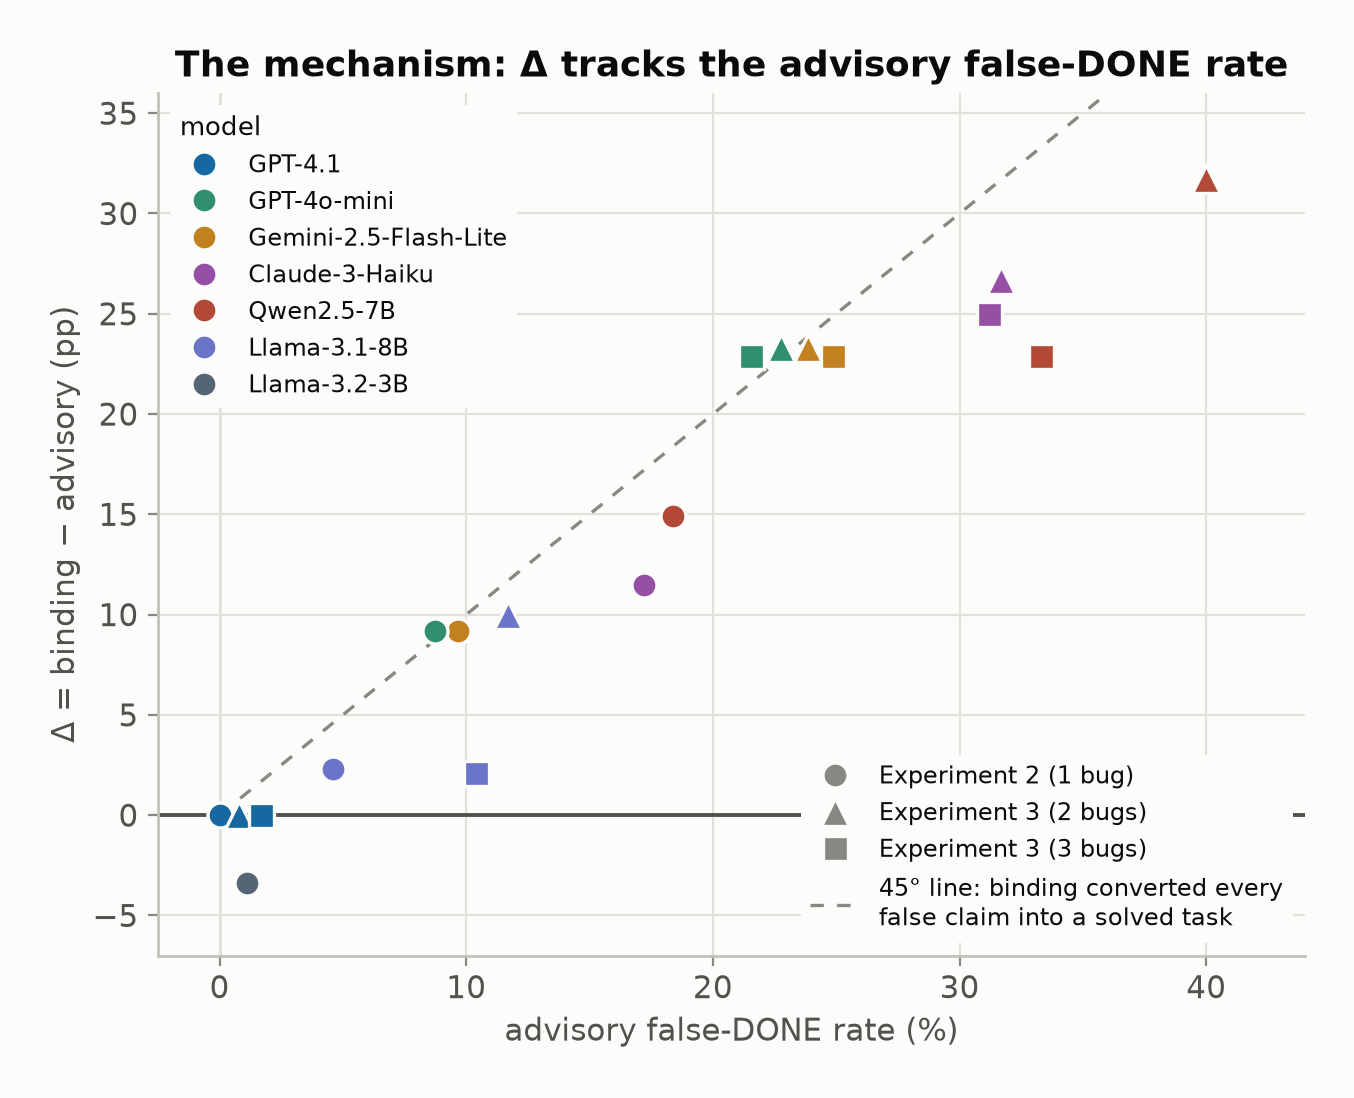
\includegraphics[width=0.8\textwidth]{fig4_mediator_scatter.png}
\caption{$\Delta$ against the advisory false-DONE rate, one point per cell across Experiments 2 and 3, with color for the model and shape for the difficulty tier. Experiment 1's two cells reproduce the Experiment 2 anchor values exactly and are present through those points. Coincident points are slightly separated for visibility, values unchanged. Drawn by \texttt{writeup\_figures/plot\_all.py} from \texttt{writeup\_figures/data/mediator\_scatter.csv}.}
\label{fig:mediator}
\end{figure}

\paragraph{What follows for practice.} The quantity that decides whether gating pays is measurable in advance. A short advisory probe that counts false-DONEs predicts the gate's value: a model that never false-claims gains nothing from the gate although it loses nothing either, a model that false-claims and can repair gains the most, and a model that fails without ever claiming needs capability, not enforcement.

\section{Limitations}

Every limitation below is drawn from the experiment ledger, and stating them here is cheaper than having a reviewer state them for us.

1. \textbf{Synthetic tasks:} The corpus is single-mutation bugs, and their compositions, in short standard-library Python functions. Organic bugs from real codebases are not represented, and whether the window sits in the same place for other task families is untested.\\
2. \textbf{The effect exists only under spec starvation:} With descriptions or docstrings visible, every model one-shots essentially every task and the modes are indistinguishable. The bare-code presentation is what makes the corpus discriminate, and this is reported as a finding about when gating matters rather than hidden as a condition, but it remains one presentation regime.\\
3. \textbf{Possible training contamination:} The seed functions are common utilities the models have likely seen. This inflates absolute success rates but not the advisory-versus-binding difference, which is what every conclusion rests on.\\
4. \textbf{The presentation was hardened after the pilots:} The spec-stripping steps were adopted in response to the dev-set ceiling, then registered before any test episode. They were not fixed in advance of seeing the pilots.\\
5. \textbf{Small discordant bases:} Experiment 1's effect rests on 8 tasks concentrated in one bug class, and Experiment 3's escalation finding rests on 4 events. The large and repeated effects, such as the window models' $\Delta$ at k1 and k2, do not share this fragility, but the fine-grained claims do.\\
6. \textbf{The ceiling is one model from one provider:} Every statement about the window's upper edge rests on GPT-4.1. A different frontier model could in principle false-claim under composition.\\
7. \textbf{Capability rank is imported, not measured:} The ladder order comes from published benchmarks combined by a fixed rule, which avoids circularity at the cost of trusting external scores.\\
8. \textbf{The difficulty axis is bug count only:} Three points were measured, at 1, 2, and 3 bugs. Harder in this program means more independent mechanical faults, not novel bug families, longer programs, or missing information of a different kind, and the composed tasks are multi-label in the bug-type breakdowns.\\
9. \textbf{Operational scars are logged:} Two Experiment 2 cells were re-run under a hard deadline after provider hangs, the checker's guard is a static filter rather than an OS-level sandbox, and one half of Experiment 3's publish gate was waived, recorded verbatim as a deviation.

\section{What this means for agent design, and reproducibility}

\paragraph{Design advice:} The practical question this program answers is not ``should agents be completion-gated'' but ``which agents should be.'' The deciding quantity is measurable in advance: run a short advisory probe and count false-DONEs. A model that never false-claims gains nothing from the gate, although gating it costs nothing and in these experiments was consistently cheaper. A model that false-claims and can repair on feedback sits in the window, and gating it buys the largest reliability gain in the program, up to 31.7 points. A model that fails without claiming sits below the window, and gating it makes things worse, so the correct response to that probe result is a stronger model or a human handoff, not enforcement. One mechanism-level lesson travels with this: escalation as implemented here is a terminal failure, and its entire measured contribution was harm at the weak edge, so a production gate should treat repeated identical failure as a handoff to a stronger authority rather than an endpoint.

\paragraph{Scale and cost of the evidence:} The three experiments comprise 2,862 committed episodes across seven models and five providers, and the total API spend for the entire program was under one US dollar. Reliability experiments of this shape are cheap enough that there is little excuse for shipping an agent harness on intuition.

\paragraph{Reproducibility:} Every number in this write-up regenerates from committed artifacts by one deterministic command per experiment, reading only the frozen episode logs, manifests, task metadata, and checker, with no API calls, and two runs produce byte-identical output. The corpus, the splits, and both composition tiers are pinned by content hashes, the predictions are locked by git tags that provably precede the data, and every deviation from plan, including the one waived gate, is recorded verbatim in an append-only experiment log. The repository is public at \url{https://github.com/kushagrab21/binding-feedback-experiment}.

\paragraph{Provenance:} The harness, scaffolding, and analysis code were built with AI assistance under execution-verified acceptance gates: every phase advanced only on raw command output audited by the author, with all deviations logged. The research questions, the registered predictions, the verification discipline, and the interpretations are the author's, and an idea-level provenance ledger for the program is published alongside the repository.

\begin{thebibliography}{9}

\bibitem{mcnemar1947}
McNemar, Q. (1947).
Note on the sampling error of the difference between correlated proportions or percentages.
\emph{Psychometrika}, 12(2), 153--157.

\bibitem{spearman1904}
Spearman, C. (1904).
The proof and measurement of association between two things.
\emph{The American Journal of Psychology}, 15(1), 72--101.

\bibitem{hendrycks2021}
Hendrycks, D., Burns, C., Basart, S., Zou, A., Mazeika, M., Song, D., and Steinhardt, J. (2021).
Measuring massive multitask language understanding.
\emph{International Conference on Learning Representations}.

\bibitem{chiang2024}
Chiang, W.-L., Zheng, L., Sheng, Y., Angelopoulos, A. N., Li, T., Li, D., Zhang, H., Zhu, B., Jordan, M., Gonzalez, J. E., and Stoica, I. (2024).
Chatbot Arena: an open platform for evaluating LLMs by human preference.
arXiv:2403.04132.

\end{thebibliography}


\end{document}
